\documentclass{article}

% Language setting
% Replace `english' with e.g. `spanish' to change the document language
\usepackage[english]{babel}

% Set page size and margins
% Replace `letterpaper' with `a4paper' for UK/EU standard size
\usepackage[letterpaper,top=2cm,bottom=2cm,left=3cm,right=3cm,marginparwidth=1.75cm]{geometry}

% Useful packages
\usepackage{amsmath}
\usepackage{graphicx}
\usepackage[colorlinks=true, allcolors=blue]{hyperref}

\title{PS6}
\author{Anais Ouedraogo}

\begin{document}
\maketitle


\section{IMdb movies rating}

I found an excel dataset in Kaggle with 250 IMDb movies and their information such as rating, budget, directors, writers, and certificates. I did not do a lot of cleanup as the data was ready to work with. I did remove invalid values or rows that had NAs. I also converted the budget column to numeric values so I can perform calculations.

The first graph (Figure 1) that I did is the line graph that shows the average budget for all movies in each year from 1921 to 2022. We can notice on the graph that in 1977 the average budget was much higher compared to other years. This might be explained by big changes in the movie industry such as Hollywood movies opening overseas.
\begin{figure}
\centering
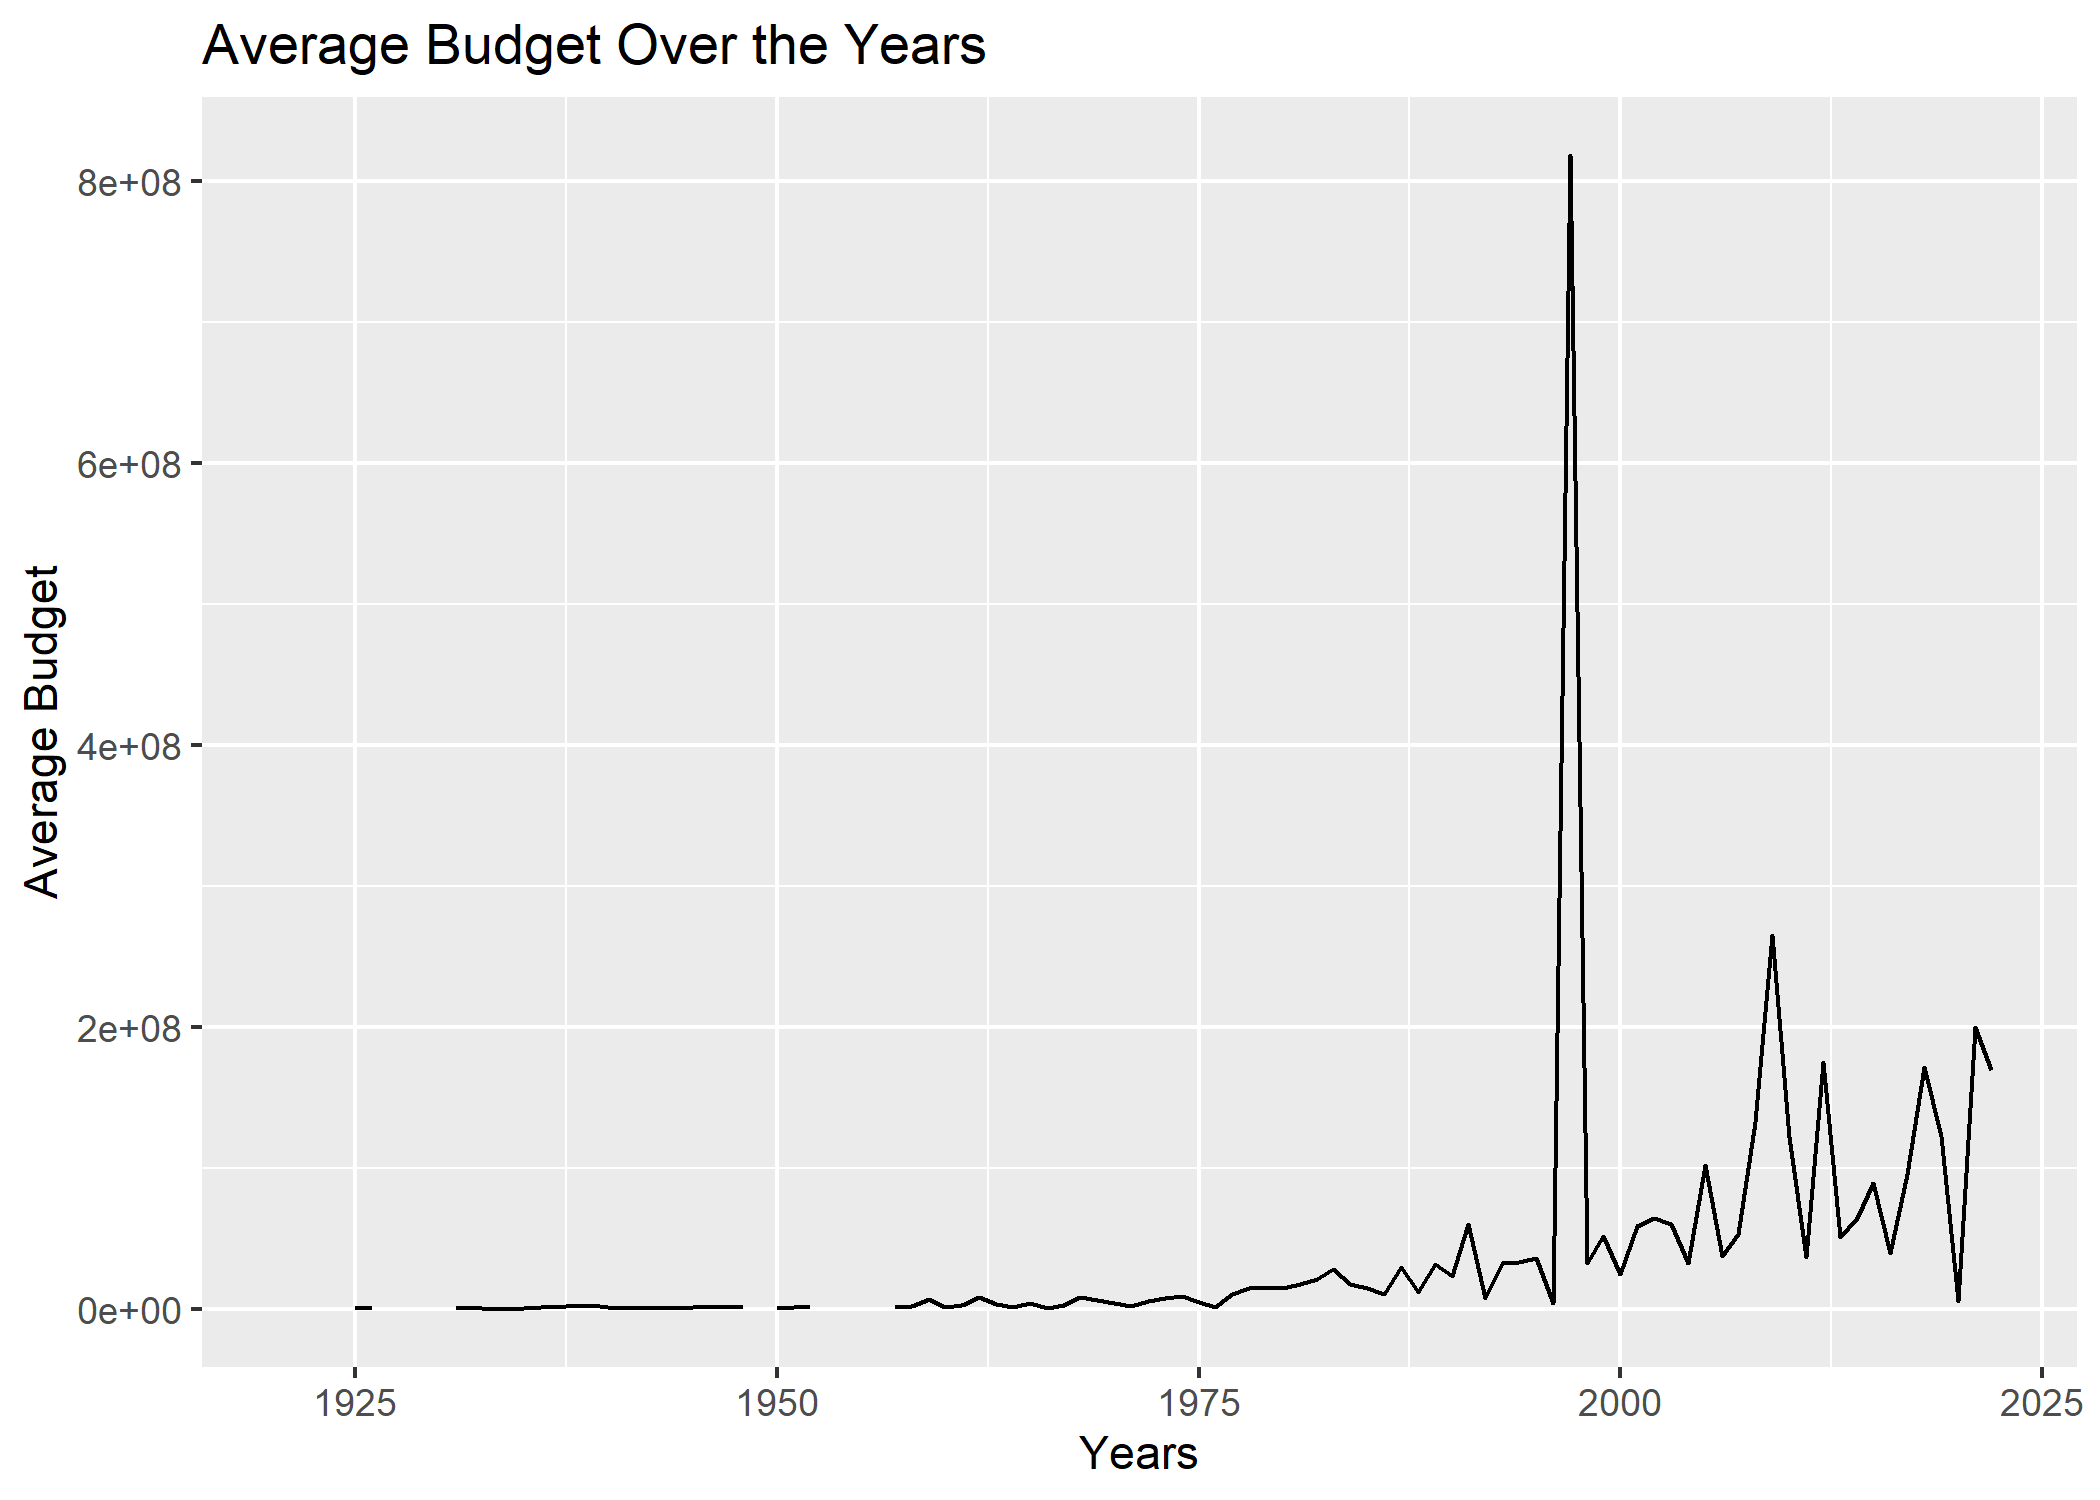
\includegraphics[width=0.8\textwidth]{PS6a_Ouedraogo.png}
\caption{\label{fig:graph1}Line chart of average movies' budget over the years.}
\end{figure}

The second graph (Figure 2) I did was a tree map to show the total budget in each genre category. We can see that the Action/Adventure/Drama has the highest total budget.
\begin{figure}
\centering
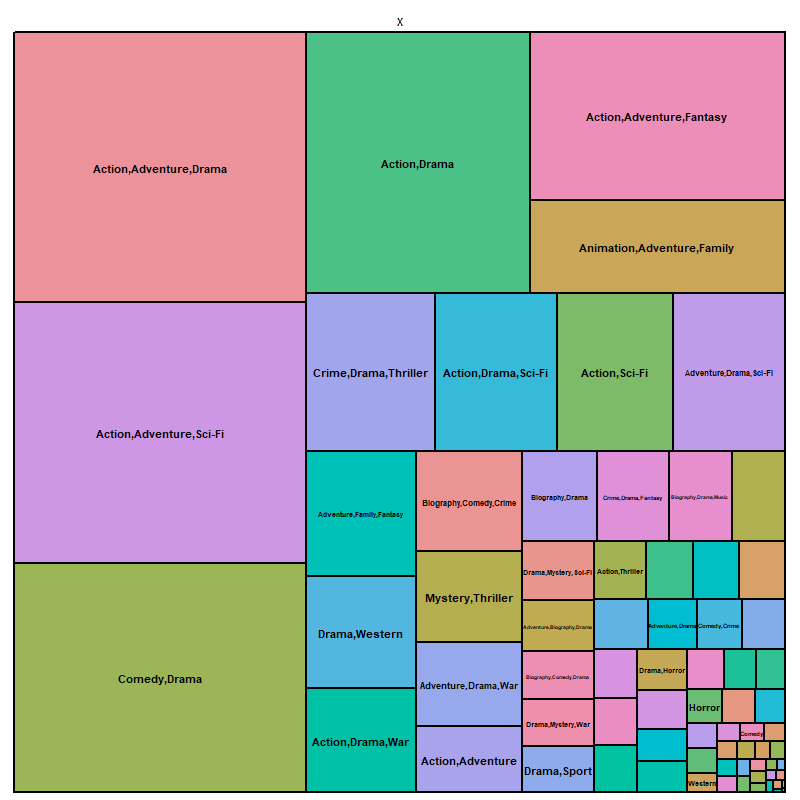
\includegraphics[width=0.8\textwidth]{PS6b_Ouedraogo.png}
\caption{\label{fig:graph2}Tree map of the total budget in each movie genre.}
\end{figure}

The third graph (Figure 3) was a bar chart that shows the different certificates and the number of movies that had a particular certificate. R was the certificate that had the highest number of movies followed by PG and PG-13.
\begin{figure}
\centering
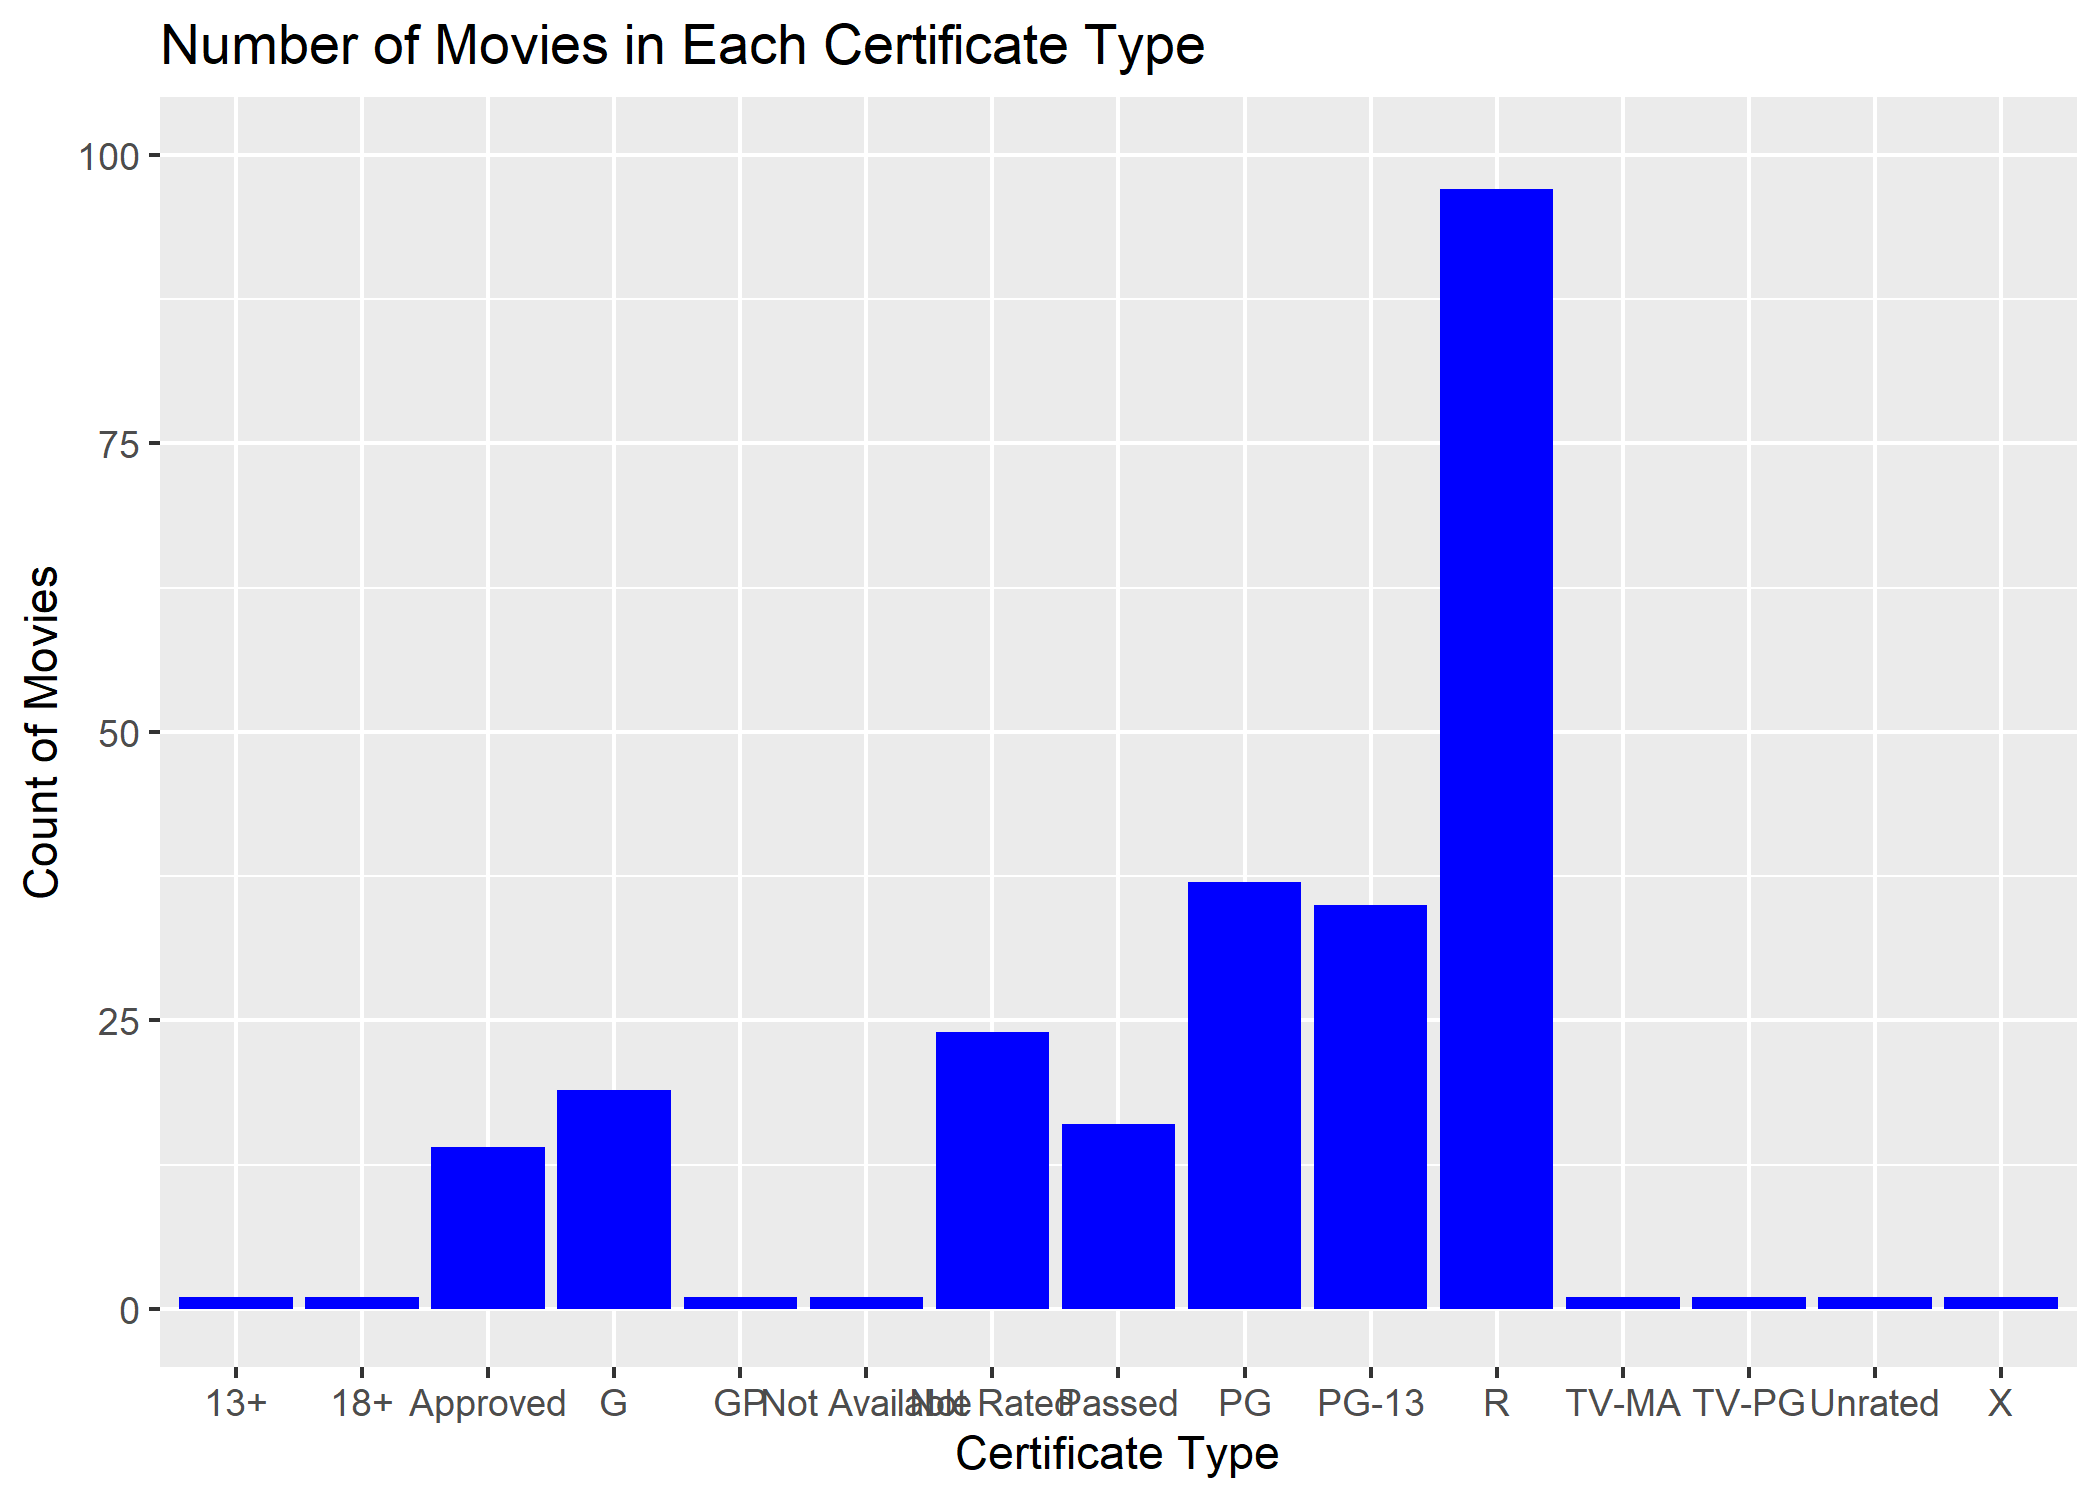
\includegraphics[width=0.8\textwidth]{PS6c_Ouedraogo.png}
\caption{\label{fig:graph3}Bar chart of the number of movies in each certificate type.}
\end{figure}

\end{document}